\section{Linear Regression}

\subsection{Part 1}
\textbf{Task:} Exclude Mont Ventoux and Pic du Midi, fit a linear regression with latitude, longitude, altitude, and discuss coefficient relevance.

\paragraph{Answer.}
Using the reduced dataset (without Mont Ventoux and Pic du Midi), the reported linear model coefficients are:
\[
\beta = [37.2650,\,-0.53396,\,0.03210,\,-0.006414]
\]
where the vector corresponds to intercept and the spatial predictors used in the model.

The reported p-values indicate that not all three spatial attributes are equally informative. In particular, longitude has a high p-value (\(\approx 0.4236\)), while latitude and altitude are more significant. Therefore, the model selection step keeps the two strongest predictors and removes the less informative one.

\subsection{Part 2}
\textbf{Task:} Build model with the two most significant attributes, predict Mont Ventoux and Pic du Midi temperatures, and include 95\% confidence intervals.

\paragraph{Answer.}
The reduced model (using the two most significant variables) reports:
\[
\text{MSE} = 0.4815989858138969
\]

Predictions and confidence intervals:
\begin{itemize}
  \item \textbf{Mont Ventoux}: true temperature \(=3.6\), predicted \(=6.1876\), 95\% CI \(=(4.3337,\ 8.0414)\).
  \item \textbf{Pic du Midi}: true temperature \(=-1.2\), predicted \(=-3.4637\), 95\% CI \(=(-8.1348,\ 1.2073)\).
\end{itemize}

Interpretation of uncertainty:
\begin{itemize}
  \item For Mont Ventoux, the measured value is outside the 95\% interval, suggesting the model under-represents this extreme case.
  \item For Pic du Midi, the measured value lies inside the 95\% interval, indicating consistency with model uncertainty for this point.
\end{itemize}

\subsection{Part 3}
\textbf{Task:} Report MSE and discuss 3D scatterplot quality.

\paragraph{Answer.}
The reported mean squared error of the second model is:
\[
\text{MSE} = 0.4815989858138969
\]

From the provided interpretation, the model quality is good overall for regular observations, but weaker for extreme stations (especially high mountain conditions). This indicates that the linear relation captures the dominant trend, while local extremes may require richer features or a non-linear model to improve fit.

The 3D scatterplot can be generated from the project code using:
\texttt{python main.py} in the \texttt{LinearRegression} folder.

\begin{figure}[h]
  \centering
  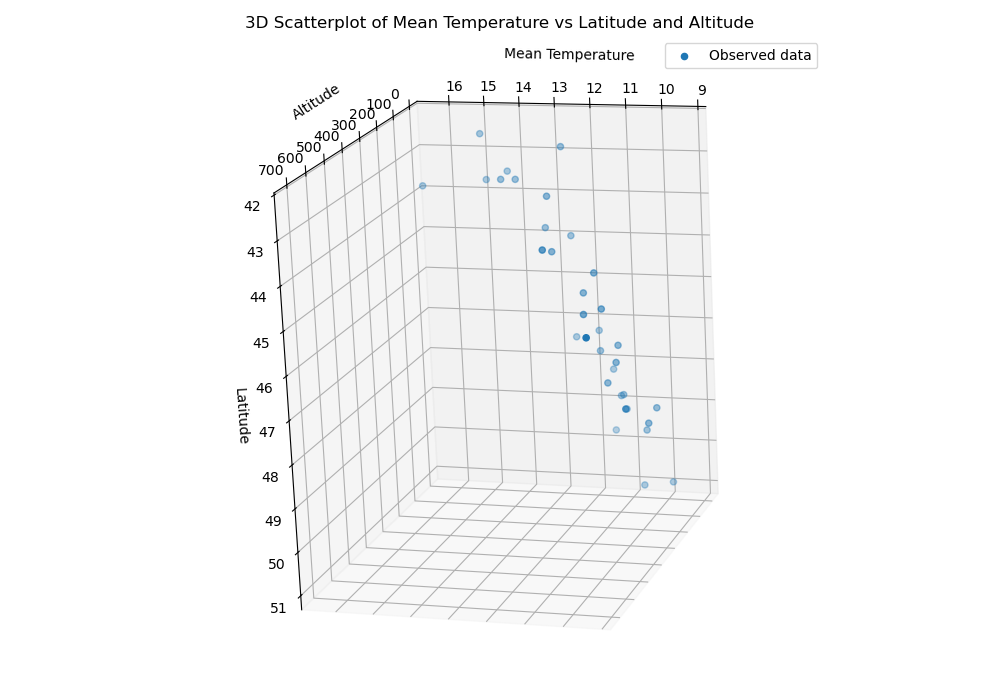
\includegraphics[width=0.78\textwidth]{figures/linear_regression_graph.png}
  \caption{Linear regression visualization from the project workflow.}
  \label{fig:linear_regression_graph}
\end{figure}
